\startchapter{Optimizing Stream Programs}
\label{chap:optimizing}

This chapter validates the premise that stream programming enables new
and powerful optimiations that are outside the reach of a traditional
compiler.  We highlight three projects in the StreamIt group:

\begin{enumerate}

\item {\it Parallelization.}  We demonstrate an end-to-end stream 
compiler that attains robust multicore performance in the face of
varying application characteristics.  As benchmarks exhibit different
amounts of task, data, and pipeline parallelism, we exploit all types
of parallelism in a unified manner in order to achieve this
generality.  Our compiler, which maps from the StreamIt language to
the 16-core Raw architecture, attains an 11x mean speedup and an 18x
maximum speedup over a single-core baseline.  {\it Project leader:}
Michael Gordon~\cite{gordon-asplos06}.

\item {\it Optimizing Linear Computations}.  We demonstrate that 
several algorithmic transformations, traditionally hand-tuned by DSP
experts, can be completely automated by the compiler.  We focus on
linear filters, where each output is an affine combination of the
inputs.  We present several optimizations of linear filters, including
algebraic simplification of adjacent filters and automatic translation
to the frequency domain.  These transformations offer an average
speedup of 5.5x and a maximum speedup of 8.0x over unoptimized
StreamIt on a Pentium~4.  {\it Project leaders:} Andrew
Lamb~\cite{lamb-pldi03,lamb-thesis} and Sitij
Agrawal~\cite{agrawal-cases05,agrawal-thesis}.

\item {\it Cache Optimizations}.   We formulate a set of cache aware 
optimizations that automatically improve instruction and data
locality.  We highlight two techniques: 1) cache aware fusion, which
combines adjacent filters while respecting instruction cache
constraints, and 2) cache aware scaling, which improves instruction
locality while respecting data cache constraints.  Our implementation
of cache aware optimizations in the StreamIt compiler yields a 3.49x
average speedup and an 88x maximum speedup over unoptimized StreamIt
on a StrongARM 1110 processor.  {\it Project leader:} Janis
Sermulins~\cite{sermulins:lctes:2005,sermulins-thesis}.

\end{enumerate}

While the author contributed to each of these projects, they are the
full-time focus of other individuals and also appear (or will appear)
in their theses.  Unlike the other chapters in this thesis, our
treatment does not aim to be comprehensive.  For more details, please
consult the papers referenced above.

\section{Parallelization}

%% Our compiler relies on two new techniques.  {\it Coarse-grained data
%% parallelism} increases the granularity of data-parallel streams to
%% match the coarse-grained nature of multicores.  It is analogous to
%% fusion of DOALL loops in the scientific domain.  {\it Coarse-grained
%% software pipelining} applies traditional instruction-scheduling
%% techniques at the level of coarse-grained actors, offering a new level
%% of scheduling freedom for stream programs.  The techniques are
%% complementary and are best when applied together.

%%%%%%%%%%%%%%%%%%%%%%%%%%%%%%%%%%%%%%%%%%%%%%%%%%%%%%%%%%

%% The first technique exploits {\it coarse-grained data parallelism} by
%% duplicating data-parallel sections across cores.  While traditional
%% data parallelism incurs excessive communication and synchronization
%% costs on multicores, our technique utilizes a program analysis to
%% coarsen the granularity of data-parallel actors and duplicate them the
%% minimum number of times needed.  The second technique, {\it
%% coarse-grained software pipelining}, leverages powerful properties of
%% the stream programming model to apply traditional
%% instruction-scheduling techniques at the level of coarse-grained
%% actors.  This increases scheduling freedom and extracts valuable
%% pipeline parallelism from the application.

%%%%%%%%%%%%%%%%%%%%%%%%%%%%%%%%%%%%%%%%%%%%%%%%%%%%%%%%%%

%% In this paper, we describe two new techniques for mapping stream
%% programs to multicores.  The first technique exploits {\it
%% coarse-grained data parallelism} by duplicating data-parallel sections
%% across cores.  While traditional data parallelism incurs excessive
%% communication and synchronization costs on multicores, our technique
%% utilizes a program analysis to coarsen the granularity of
%% data-parallel actors and duplicate them the minimum number of times
%% needed.  The second technique, {\it coarse-grained software
%% pipelining}, leverages powerful properties of the stream programming
%% model to apply traditional instruction-scheduling techniques at the
%% level of coarse-grained actors.  This increases scheduling freedom and
%% extracts valuable pipeline parallelism from the application.

%% We have implemented these techniques in the StreamIt compiler,
%% targeting the 16-core Raw architecture.  Coarse-grained data
%% parallelism offers a 9.9x mean speedup over a single-core baseline,
%% while coarse-grained software pipelining offers a 7.7x speedup.
%% Combining the techniques yields the best results, achieving a 11.2x
%% speedup over a single core and 1.84x over our previous work.

Despite the abundance of parallelism in stream programs, it is
nonetheless a challenging problem to obtain an efficient mapping to a
multicore architecture.  Often the gains from parallel execution can
be overshadowed by the costs of communication and synchronization.  In
addition, not all parallelism has equal benefits, as there is
sometimes a critical path that can only be reduced by running certain
actors in parallel.  Due to these concerns, it is critical to leverage
the right combination of task, data, and pipeline parallelism while
avoiding the hazards associated with each.

\begin{figure}[t]
\centering
\psfig{figure=parallelism.eps,width=2.1in}
\caption[Types of parallelism in stream programs]{Types of parallelism
  in stream programs.  Task parallelism exists between filters in a
  common splitjoin; pipeline parallelism exists between filters in a
  producer/consumer relationship; and data parallelism exists between
  separate instances of a stateless
  filter.\protect\label{fig:parallelism}}
\end{figure}

Task parallelism refers to pairs of actors that are on different
parallel branches of the original stream graph, as written by the
programmer.  That is, the output of each actor never reaches the input
of the other (see Figure~\ref{fig:parallelism}).  In stream
programs, task parallelism reflects logical parallelism in the
underlying algorithm.  It is easy to exploit by mapping each task to
an independent processor and splitting or joining the data stream at
the endpoints.  The hazards associated with task parallelism are the
communication and synchronization associated with the splits and
joins.  Also, as the granularity of task parallelism depends on the
application (and the programmer), it is not sufficient as the only
source of parallelism.

Data parallelism refers to any actor that has no dependences between
one execution and the next.  Such ``stateless'' actors\footnote{A
  stateless actor may still have read-only state.}  offer unlimited
data parallelism, as different instances of the actor can be spread
across any number of computation units.  However, while data
parallelism is well-suited to vector machines, on coarse-grained
multicore architectures it can introduce excessive communication
overhead.  Previous data-parallel streaming architectures have focused
on designing a special memory hierarchy to support this
communication~\cite{imagine03ieee}.  However, data parallelism has the
hazard of increasing buffering and latency, and the limitation of
being unable to parallelize actors with state.

Pipeline parallelism applies to chains of producers and consumers that
are directly connected in the stream graph.  In our previous
work~\cite{streamit-asplos}, we exploited pipeline parallelism by
mapping clusters of producers and consumers to different cores and
using an on-chip network for direct communication between actors.
Compared to data parallelism, this approach offers reduced latency,
reduced buffering, and good locality.  It does not introduce any
extraneous communication, and it provides the ability to execute any
pair of stateful actors in parallel.  However, this form of pipelining
introduces extra synchronization, as producers and consumers must stay
tightly coupled in their execution.  In addition, effective load
balancing is critical, as the throughput of the stream graph is equal
to the minimum throughput across all of the processors.

In this section, we describe a robust compiler system that leverages
the right combination of task, data, and pipeline parallelism to
achieve good multicore performance across a wide range of input
programs.  Because no single type of parallelism is a perfect fit for
all situations, a unified approach is needed to obtain consistent
results.  Using StreamIt as our input and targeting the 16-core Raw
architecture, our compiler demonstrates a mean speedup of 11.2x over a
single-core baseline.  This also represents a 1.84x improvement over
our original approach~\cite{streamit-asplos}.

\subsection*{Parallelization Algorithm}

\begin{figure}[t]

\begin{minipage}{0.3\textwidth}
\centering
\psfig{figure=filterbank.eps,width=1.6in}
\end{minipage}
\hspace{0.1in}
\begin{minipage}{0.3\textwidth}
\centering
\psfig{figure=filterbank-fine.eps,width=2.2in}
\end{minipage}
\hspace{0.4in}
\begin{minipage}{0.3\textwidth}
\centering
\psfig{figure=filterbank-coarse.eps,width=1.6in}
\end{minipage}

~ \\
\begin{minipage}{0.3\textwidth}
\centering
\mbox{{\small (a) Original}}
\end{minipage}
\hspace{0.1in}
\begin{minipage}{0.3\textwidth}
\mbox{{\small (b) Fine-grained data parallelism}}
\end{minipage}
\hspace{0.4in}
\begin{minipage}{0.3\textwidth}
\hspace{-14pt}\mbox{{\small (c) Coarse-grained data parallelism}}
\end{minipage}

\centering
\caption[Exploiting data parallelism in the FilterBank
  benchmark]{Mapping a simplified version of the FilterBank benchmark
  for execution on four cores.  The original stream graph is shown in
  (a), while a conventional mapping is shown in (b).  Our technique
  coarsens the graph and introduces the minimal parallelism needed, as
  shown in (c).\protect\label{fig:filterbank}}

\end{figure}

We illustrate our technique by way of an example: we discuss how to
map a simplified version of our FilterBank benchmark (see
Figure~\ref{fig:filterbank}a) to a four-core machine.  The complete
details of our algorithm are available
elsewhere~\cite{gordon-asplos06}.

\paragraph*{Previous Practice: Fine-Grained Data Parallelism}  Perhaps 
the most common approach to parallelization is to identify loops that
can be run in a data-parallel (DOALL) style.  Such loops can be
annotated by the programmer using OpenMP; they are also the most
common parallelization target of production compilers.  For example,
the Intel C Compiler includes an optional flag to detect and
parallelize data-parallel loops.  In the case of FilterBank, this may
seem like a promising approach, as all the filters are stateless and
the implicit loops surrounding them can be run in a data-parallel
manner.  Figure~\ref{fig:filterbank}b illustrates such a mapping.

Unfortunately, on a coarse-grained multicore architecture, it is
hardly profitable to parallelize each individual filter due to the
communication and synchronization overheads incurred.  When we target
the 16-core Raw architecture, this approach offers only a 1.4x mean
speedup over a single core.  This represents an upper bound on the
speedups attainable using standard techniques.  In practice, for
reasons explained in Section~\ref{sec:filters}, a production C
compiler would achieve even smaller speedups due to the inherent
difficulties of proving that filters are data-parallel.

\paragraph*{First Innovation: Coarse-Grained Data Parallelism}  The
overheads of fine-grained data parallelism can be drastically reduced
by performing two novel transformations.  First, the granularity of
the stream graph is coarsened via filter {\it fusion}, a
transformation in which two neighboring filters are statically
scheduled and inlined into a single
filter~\cite{streamit-asplos,sermulins:lctes:2005}.  We fuse
neighboring stateless filters as much as possible so long as the
resulting filter remains stateless, ensuring that it is still amenable
to data parallelism.

Second, we data-parallelize the coarsened filters, but only by the
amount necessary to complement existing task parallelism in the stream
graph.  That is, for filters that are already embedded in a splitjoin,
we parallelize each filter so that the total splitjoin width covers
all of the cores, rather than data-parallelizing each branch of the
splitjoin to cover all of the cores.  By reducing the width of the
scatter and gather stages, we reduce the communication and
synchronization overhead incurred by data parallelism.

Figure~\ref{fig:filterbank}c shows an example of our
transformations on the FilterBank benchmark.  The coarsening stage
fuses all of the pipelines together with the exception of the BandStop
filter, which is not fused because it performs peeking on its input
channel.  Communication with peeking represents a case where some data
items are reused between successive firings of a filter, which would
translate to internal state if the buffer were to be inlined into a
fused filter.  Following coarsening, the parallelization stage
replicates the Adder filter across all four of the target cores.
However, the other filters are split only two ways, due to the
presence of task parallelism between alternate branches of the
splitjoin.  Applying this strategy across our benchmark suite offers a
speedup of 9.9x relative to a single core.

These transformations are out-of-reach of traditional compilers.  In
an imperative language, the analog of graph coarsening is to
selectively fuse loops so long as no new loop-carried dependences are
introduced.  The analog of task-conscious data parallelism is to
analyze the entire program for other threads that might be running
concurrently, and to introduce only as much parallelism as is needed
to complement the other threads.  We rely on the properties of the
stream programming model to make these transformations tractable.

\begin{figure}[t]
\centering
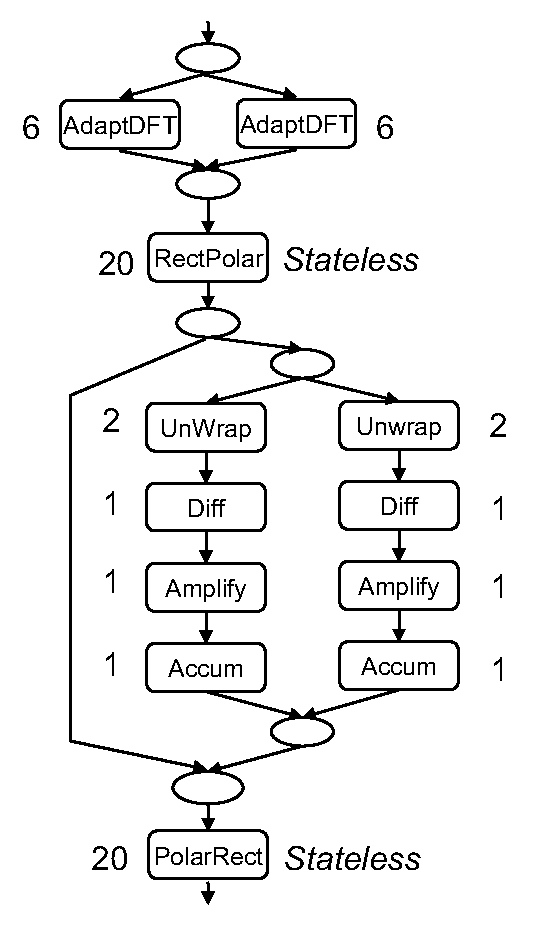
\psfig{file=vocoder.eps,width=2in}
\caption[Simplified subset of the Vocoder benchmark]{Simplified subset
  of the Vocoder benchmark.  Nodes are annotated with the amount of
  work that they perform per steady state.\protect\label{fig:vocoder}}
\end{figure}

\begin{figure}[t]
\centering
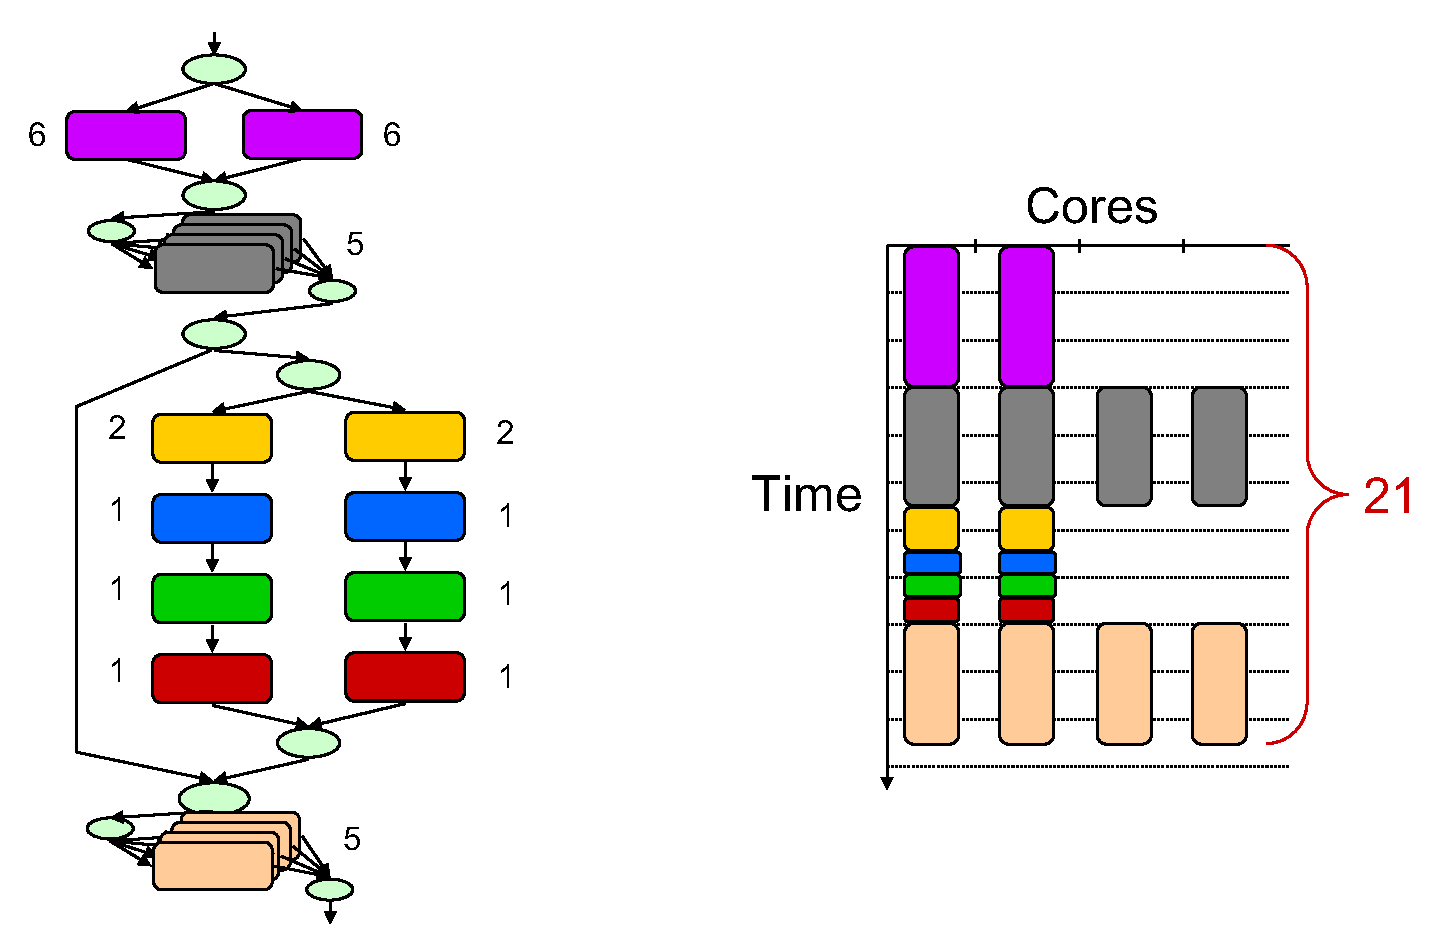
\psfig{file=vocoder-data.eps,width=4.5in}
\caption[Coarse-grained data parallelism applied to
  Vocoder]{Simplified vocoder mapped with data parallelism.  In the
  stream graph (left), stateless nodes are replicated but stateful
  nodes remain untouched.  An execution trace (right) requires 21
  units per steady state.\protect\label{fig:vocoder-data}}
\end{figure}

\begin{figure}[t]
\centering
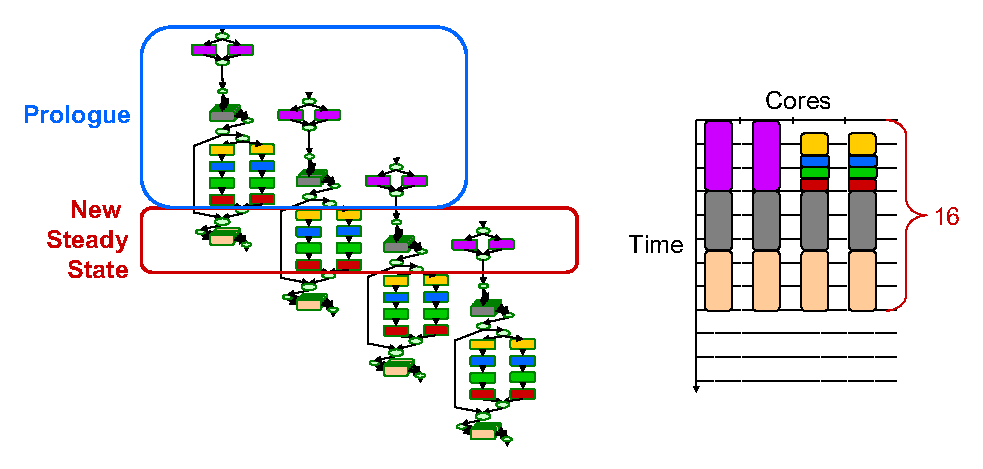
\psfig{file=vocoder-swpipe.eps,width=6in}
\caption[Coarse-grained software pipelining applied to
  Vocoder]{Simplified vocoder mapped with coarse-grained software
  pipelining.  By unrolling multiple executions of the stream graph
  (left), stateful nodes can run in parallel with other nodes during
  the steady state.  An execution trace (right) requires 16 units per
  steady state, an improvement over plain data parallelism.
  \protect\label{fig:vocoder-swpipe}}
\end{figure}

%% \begin{figure}[t]
%% \centering
%% \psfig{figure=asplos06/vocoder.eps,width=4.2in}
%% \vspace{-24pt}
%% \caption{Stream graph for a simplified subset of our Vocoder
%% benchmark.  Following a set of sliding DFTs, the signal is converted
%% to polar coordinates.  Node {\tt S2} sends the magnitude component to
%% the left and the phase component to the right.  In this simplified
%% example, no magnitude adjustment is needed.\label{fig:vocoder}}
%% \vspace{-12pt}
%% \end{figure}

\paragraph*{Second Innovation: Coarse-Grained Software Pipelining} While 
coarse-grained data parallelism is effective for parallelizing
stateless computations, it does nothing to help with computations that
retain state, either within filters or within feedbackloops.  For
example, the Vocoder benchmark (simplified subet shown in
Figure~\ref{fig:vocoder}) contains a significant fraction of stateful
filters.  While two of the filters can be data-parallelized, there
remain large gaps in the execution schedule (see
Figure~\ref{fig:vocoder-data}).

To run stateful computations in parallel with each other, we exploit
pipeline parallelism.  We take the concept of software pipelining,
well-understood in the context of instruction scheduling, and apply it
in the context of an entire stream graph.  As illustrated in
Figure~\ref{fig:vocoder-swpipe}, this technique involves unrolling the
execution of the graph into two stages.  In the first stage, a
prologue schedule establishes buffering in the data channels.  Then,
in the steady state, the filters are decoupled and can execute in any
order, writing intermediate results to the buffers.  Compared to
exploiting only coarse-grained data parallelism, this technique offers
large gains for our stateful benchmarks (1.7x for Vocoder, 1.9x for
Radar).  Together with coarse-grained data parallelism, it offers an
11.2x speedup over a single core across our benchmark suite.

Coarse-grained software pipelining is also beyond the reach of
traditional compilers.  Rather than pipelining individual
instructions, it represents the pipelining of entire procedures.  This
involves reordering large pieces of the program.  The stream
programming model makes such a transformation feasible by exposing the
stable flows of data between long-running actors.

\subsection*{Experimental Evaluation}

%\begin{figure}
%\centering
%\psfig{figure=asplos06/raw-diagram.eps,width=3in}
%\caption{Block diagram of the Raw architecture.
%\protect\label{fig:raw-diagram}}
%\end{figure}

We target the Raw microprocessor~\cite{raw10,raw}, a tiled array of 16
cores with a programmable mesh interconnect.  Though Raw has been
implemented in silicon, we generate results with the btl simulator,
augmented with 16 streaming DRAM controllers (providing enough
bandwidth to saturate both directions of a Raw port).  In this
configuration, one can obtain higher throughput in streaming data from
the off-chip memory than from a core's local data cache.  Thus, our
implementation elects to buffer all streaming data off-chip.  However,
when targeting an architecture with more modest off-chip memory
bandwidth, the stream buffers could reside completely in on-chip
memory.

\begin{figure}[t]
\centering
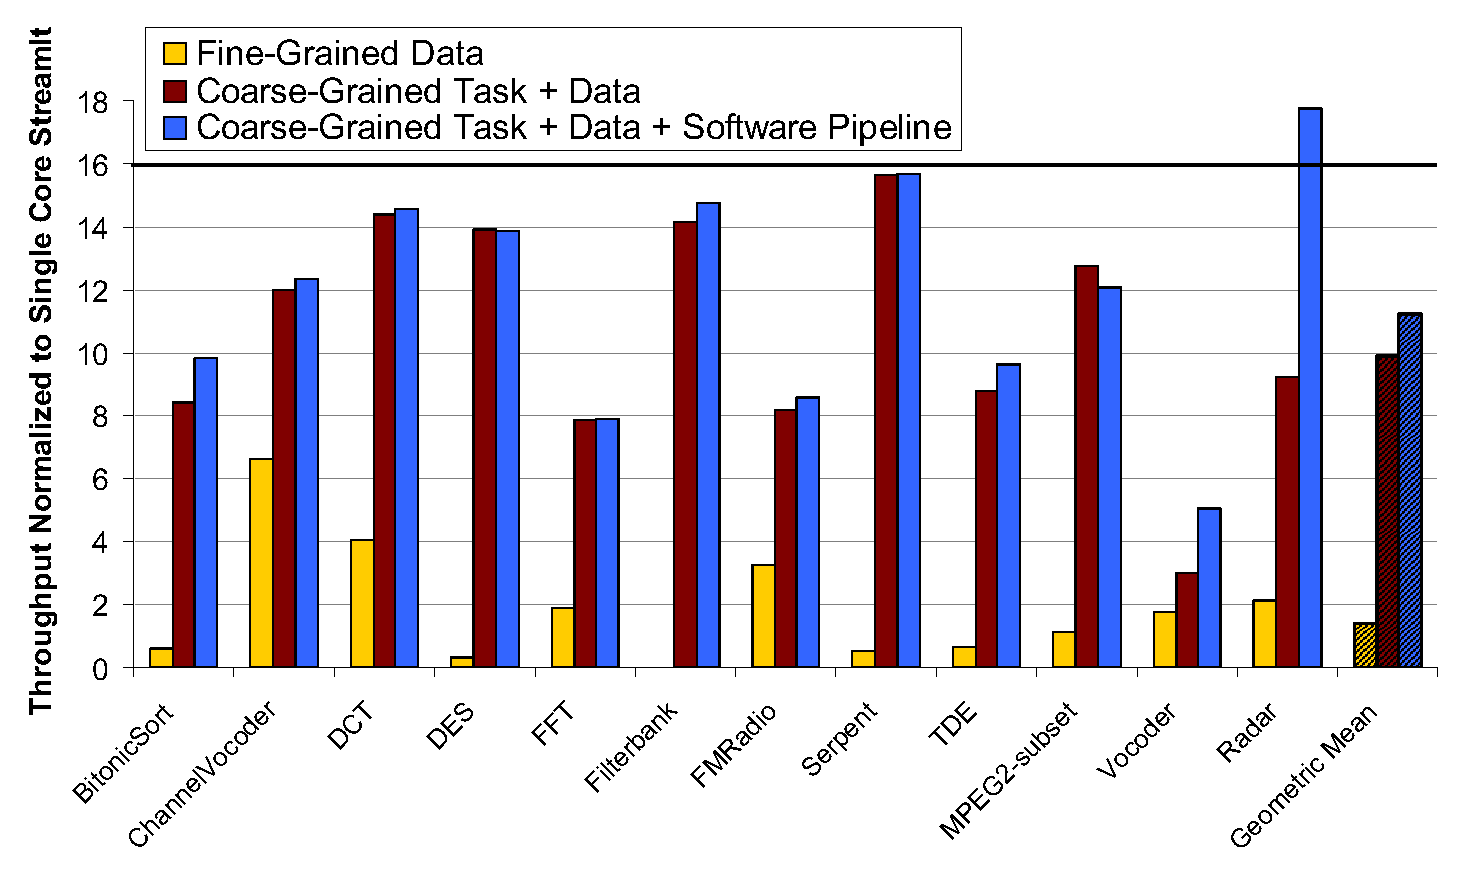
\psfig{file=par-results.eps,width=\textwidth}
\caption[Parallelization results]{Parallelization results on the
  16-core Raw processor.\protect\label{fig:par-results}}
\end{figure}

A summary of our results appears in Figure~\ref{fig:par-results}.  We
show the speedup offered by the three techniques mentioned:
fine-grained data parallelism, the previous standard; coarse-grained
data parallelism, which also leverages the existing task parallelism
in the stream graph; and coarse-grained software pipelining, which
runs as a post-pass to coarse-grained data parallelism.  Our baseline
is StreamIt executing on a single core, which (in the case of Raw) has
been shown to outperform hand-written C implementations on a single
core~\cite{raw_isca}.  While coarse-grained data parallelism performs
well (attaining a mean speedup of 9.9x), the most robust performance
comes by adding coarse-grained software pipelining (which attains a
mean speedup of 11.2x).  As expected, software pipelining mostly
benefits the stateful benchmarks, Vocoder and Radar.  There is a
super-linear speedup in Radar because reordering operations were moved
from the compute core to the network.

%% \begin{figure}[t]
%% \centering
%% \psfig{figure=asplos06/benchchar.eps, width=6.15in}
%% \caption{Benchmark descriptions and characteristics.
%% \protect\label{fig:benchchar}}
%% \end{figure}

%% \begin{figure}[t]
%% \centering
%% \psfig{figure=asplos06/thruput.eps, width=6.1in}
%% \caption{Throughput speedup comparison and Task + Data + Software
%% Pipelining performance results.  \protect\label{fig:thruput}}
%% \end{figure}

%% \begin{figure}[t]
%% \centering
%% \psfig{figure=asplos06/maingraph.eps, width=6.5in}
%% \caption{Task, Task + Data, Task + Software Pipelining, and Task +
%% Data + Software Pipelining normalized to single core.
%% \protect\label{fig:main_comp}}
%% \end{figure}

%% \begin{figure}[t]
%% \centering
%% \psfig{figure=asplos06/fine_data.eps, width=4.5in}
%% \caption{Fine-Grained Data Parallelism normalized to single core.
%% \protect\label{fig:fine_data}}
%% \end{figure}

%% \begin{figure}[t]
%% \centering
%% \psfig{figure=asplos06/vs_space_graph.eps, width=4.5in}
%% \caption{Task + Data + Software Pipelining normalized to Hardware Pipelining.
%% \protect\label{fig:vs-space}}
%% \end{figure}

\section{Optimizing Linear Computations}

The design flow for digital signal processing applications typically
contains three steps.  First, application designers specify a block
diagram of the computation, drawing on rich software libraries to
prototype its behavior in an environment such as MATLAB.  Once the the
functionality has been fixed, the second step is performed by digital
signal processing (DSP) experts, who inspect the global structure of
application and perform many domain-specific optimizations to reduce
the overall processing requirements while preserving the basic
input/output relationship.  Finally, once the mathematical algorithms
have been determined, a software engineer implements those algorithms
in a low-level language such as C to obtain the final product.

In order to reduce the cost of this development process, a long-term
goal of the computer science community has been to generate efficient
and deployable code from a high-level, functional specification of the
program.  In order to achieve this goal, the expertise of DSP experts
must be encapsulated into the tool.  While library generators such as
Spiral~\cite{Spiral-SI}, FFTW~\cite{FFTW-SI}, and
ATLAS~\cite{ATLAS,ATLAS-Sparsity-SI} can automatically derive and
optimize specific classes of DSP kernels, programmers must integrate
these libraries into their development process rather than having the
compiler automatically recognize and transform the original code.  Our
goal is to invent and adapt domain-specific optimizations in the
context of the StreamIt language, so as to provide a unified
development environment that can express the full functionality of the
application while automatically applying deep optimizations to the
specific code sections where they apply.

\begin{figure}[t]
% TODO: 
%(a) Software FM radio with Equalizer
%(b) After linear combination
%(c) After translation to the frequency domain
\caption[Example optimization of linear filters]{Example optimization
  of linear filters.  Our software FM radio benchmark contains an
  equalizer in which all filters are linear.  These filters can be
  algebraically simplified into a single filter and then translated
  into the frequency domain. \protect\label{fig:equalizer}}
\end{figure}

Our focus in the current work is the optimization of {\it linear}
computations, which are the most common target of DSP experts.  Linear
filters are those in which each output is an affine combination of the
inputs.  Examples include finite impulse response (FIR) filters,
compressors, expanders and signal processing transforms such as the
discrete Fourier transform (DFT) and discrete cosine transformation
(DCT).  We also describe the optimization of linear statespace
filters, a generalization of linear filters that maintain internal
states.  In a linear statespace filter, each each output is an affine
combination of the states and the inputs, and each state is also
updated in an affine fashion.  An infinite impulse response (IIR)
filter is an example of a linear statespace filter.

Figure~\ref{fig:equalizer} illustrates an example of linear
optimizations as applied to our software radio benchmark.  The radio
contains an equalizer, which was specified by the designer in a simple
but inefficient manner.  Each frequency band is processed in a
separate branch of a splitjoin, and each branch contains a successive
high-pass and low-pass filter to accomplish a band-pass functionality.
While this representation of the algorithm allows it to be easily
understood and maintained, it perfoms many redundant computations.  In
practice, because all of the components of the equalizer are linear,
they can be collapsed into a single filter that performs far fewer
computations.  Furthermore, as that filter is performing a sliding
window computation, it can be converted into the frequency domain to
reduce the asymptotic processing requirements from $O(n^2)$ to $O(n
\log n)$.  Both of these transformations require deep inter-procedural
analysis and are far beyond the reach of traditional compilers.
However, using a stream programming model, we can robustly automate
both steps of the optimization process.

In the rest of this section, we provide an overview of our linear
optimization techniques.  We describe how to extract a linear
representation from the code in a StreamIt filter, how to
algebraically simplify adjacent linear filters, and how to translate
linear filters into the frequency domain.  We also describe
optimizations for linear statespace filters, including removal of
redundant states and reduction of the number of parameters.  We give a
procedure for determining which optimizations to apply to a given
program, and we evaluate the optimizations in the StreamIt compiler.
The average speedup obtained is 4.5x, with a maximum of 8.0x.

\subsection*{Extracting a Linear Representation}

\begin{figure}[t]
% TODO: linear extraction from statespace talk
\caption[Extracting a linear representation]{Extracting a linear
  representation from the code inside a filter's work
  function.\protect\label{fig:extraction}}
\end{figure}

Rather than directly manipulating the code inside a filter's work
function, our linear optimizations rely on an abstract representation
in which linear filters are represented by a set of matrices.
Figure~\ref{fig:extraction} gives an example of this representation
for an IIR filter.  The StreamIt compiler automatically extracts this
representation using a symbolic execution of the filter's work
function.  The basic idea is to execute a complete invocation of the
function just like a normal interpreter, except that instead of
assigning values to the states and input items, these quantities are
left as free variables and tracked throughout the execution.  If the
interpreter encounters any branches or conditionals that depend on
free variables, then the analysis is aborted and the node is deemed
non-linear.  Otherwise, when execution completes, a symbolic
expression has been established for every state variable and every
value pushed to the output tape.  If all of these expressions are an
affine function of the free variables, then linear analysis has
succeeeded and the linear representation is built.  A more precise
description of this analysis, including support for innocuous branches
that do not affect the linear representation, is described
elsewhere~\cite{lamb-pldi03}.

Of course, it would also be possible for programmers to specify the
linear representation directly rather than relying on the compiler to
extract it from the code.  If programmers prefer this approach, then
they could develop a generic linear filter in StreamIt and call it as
a library.  However, we believe that it is valuable to support
automatic recognition of optimization targets, as otherwise the
programmer needs to be knowledgeable of every potential optimization
and annotate the code accordingly.

\subsection*{Alebraic Simplification of Adjacent Linear Filters}

\begin{figure}[t]
% TODO: simple combination picture
\caption{Algebraic simplification of adjacent linear filters.\protect\label{fig:combination}}
\end{figure}

\begin{figure}[t]
% TODO: IIR + decimator with flops reducation
\caption{Example simplification of an IIR filter and a decimator.\protect\label{fig:combination-example}}
\end{figure}

If neighboring filters in the stream graph both perform a linear
computation, then that section of the stream graph can be collapsed
into a single linear filter.  The most simple case of this
transformation is illustrated in Figure~\ref{fig:combination}, where
two stateless filters are communicating in a pipeline.  Given the
computation matrix for each filter, the output of the entire pipeline
can be represented as a matrix product.  Because each of the matrices
is known at compile time, the matrix product can also be evaluated at
compile time.  This offers the potential for large performance gains.
For example, if both matrices are square (representing filters that
read the same number of items as they write) and there is no peeking
involved, then the output matrix will be the same size as each of the
input matrices, reducing the computation by a factor of two.  Larger
gains are possible if the communication rate between the filters is
larger than that of the end-to-end pipeline.  Conversely, if the
communication rate between the filters is lower than the overall
pipeline, it is possible for this transformation to to increase the
computation requirements; as described later, this hazard is avoided
by our automatic selection algorithm.  In our experimental evaluation,
combining filers wherever possible (even when detrimental) leads to a
2.1x average performance improvement, with a maximum improvement of
5.0x.
% note: if peeking involved, we currently do some re-computation in
% the linear formulation, losing some gains.  this should be re-gained
% in the linear statespace formulation, though not evaluated
% completely.

We have extended the simple idea of algebraic simplification to handle
the general case, hiding many complexities from the
user~\cite{agrawal-cases05}.  To perform the matrix multiplication
in Figure~\ref{fig:combination}, the output rate of the first filter
must match the input rate of the second filter.  In cases where this
is not true in the program, the analysis expands each linear
representation to encompass multiple executions of the original
filter.  In addition to collapsing pipelines, we have also developed
complete combination rules to handle the other StreamIt language
constructs: splitjoins and feedbackloops.  Splitjoins introduce
complexity due to the reordering in the splitters and joiners, as well
as implicit buffering that may be involved due to mis-matched I/O
rates along alternate branches.  Feedbackloops introduce complexity
because of the initial items enqueued on the backward path of the
feedback loop; in addition, the periodicity of the entire feedbackloop
may be coarser than the periodicity of its components, requiring
further expansion and analysis by the compiler.  The presence of
sliding window operations (or peeking) also adds complexity to all of
the combination rules; in our general formulation, the peeked data
items are converted into states in the filter.

By automating the combination of linear filters, we allow the
programmer to maintain a natural expression of the algorithm.
Figure~\ref{fig:combination-example} illustrates an example
combination of an IIR filter with a decimator, reducing the total
number of operations by 25\%.  This optimization opportunity is not
obvious to non-experts due to the state retained by the IIR filter.
Also, even when the programmer understands that linear combination is
possible, it may be untractable to manage of all of the details and to
maintain the code following the transformation.  This effect is
especially important in the context of software libraries, where the
final application may contain filters that were authored by many
different developers.  The compiler can perform this analysis across
module boundaries, synthesizing an efficient implementation while
preserving a modular development style.

\subsection*{Optimization of a Single Linear Filter}

In addition to optimizing groups of linear filters, it is possible to
improve the execution of a single linear filter at a time.  Stateless
filters can be mapped into the frequency domain, while stateful
filters are subject to state removal and parameter reduction.  These
transformations are generally applied after algebraic simplification.

\begin{figure}[t]
% todo: mapping to frequency
\caption{Mapping linear filters into the frequency domain.\protect\label{fig:freq}}
\end{figure}

\paragraph*{Mapping into the Frequency Domain}  Filters that perform a 
sliding window computation, such as FIR filters, are equivalent to a
convolution of the filter coefficients with the input tape.  This
means that they are amenable to a classic transformation in single
processing, whereby the computation is mapped from the time domain
into the frequency domain.  As illustrated in Figure~\ref{fig:freq},
this consists of wrapping the filter in an FFT and inverse FFT, and
changing the convolution into a vector-vector multiply.
Asymptotically, this reduces the computation requirements from
$O(n^2)$ to $O(n \log n)$, where $n$ is the size of FFT (which can be
set by the compiler).  In our experiments, translating each filter
into the frequency domain (even when detrimental) leads to an average
speedup of 3.8x and a maximum speedup of 8.0x.
% note: the 3.8x speedup is either with or without doing linear
% combination first (they both round to 3.8x)

While this transformation is well-understood and can also be done by
hand, there are benefits to automating it in the compiler.  The size
of the FFT can be automatically selected and complex startup
conditions can be handled automatically.  Also, there are cases where
it is not profitable to translate to the frequency domain (for
example, if the peek window is too small, or if the filter decimates
items in addition to peeking), or where conversion is profitable only
following linear combination.  By coupling the translation algorithm
with our optimization selection algorithm (described later), the
programmer does not need to worry about when to apply the
transformation.

\paragraph*{Removing States}  Linear statespace filters maintain and
update a set of internal states on each time step.  However,
especially following combination with adjacent nodes, it is possible
that some of these states could be redundant; that is, their values
could be fully derived from other states in the filter.  It is
beneficial to remove any redundant states, both for memory savings and
to eliminate redundant computations that update the states.

We have adapted a simple algorithm that guarantees to identify and
remove all of the redundant states in a filter~\cite{Mayne}.  While
this algorithm was previously known by the signal processing
community, to our knowledge this is its first application in an
optimizing compiler.  The algorithm works by constructing augmented
matrices from the filter's representation
(Figure~\ref{fig:extraction}), and by reducing these matrices to a
special row-echelon form.

\begin{figure}[t]
% TODO: figure of state removal and parameter reduction from CASES
\caption{Example of state removal and parameter reduction.\protect\label{fig:states}}
\end{figure}

An example of state removal appears in Figure~\ref{fig:states}.  The
analysis detects that the two states {\tt x1} and {\tt x2} were always
scaled proportionately, so they can be combined into a single state
{\tt x}.  This reduced the computational requirements of the filter
from 9 FLOPs per execution to 5 FLOPs per execution.

\paragraph*{Reducing the Number of Parameters}  After removing as 
many states as possible, additional computations can be eliminated by
transforming the filter's linear representation into one with fewer
non-zero, non-one entries (termed parameters).  Each coefficient that
is converted to a zero serves to eliminate a multiplication and
addition operation per execution of the filter, while each coefficient
that is converted to a one serves to eliminate a multiplication.  

We automated parameter reduction by starting with a known signal
processing technique~\cite{Ackermann/Bucy} and reformulating it in the
context of StreamIt.  As with the state removal algorithm, the number
of parameters in a linear statespace filter can be reduced using a
systematic sequence of matrix operations.  However, compared to state
removal, there are looser guarantees on the optimality of the final
system~\cite{agrawal-cases05}.

An example of parameter reduction is illustrated in
Figure~\ref{fig:states}.  Following the transformation, the state
variable $x$ assumes a value that is twice as large as the original
(at any given point of execution).  However, this change does not
affect the output of the filter, as the other coefficients are
compensated accordingly.  The transformation enables two coefficients
two change to a value of 1, thereby eliminating two multiplication
operations and reducing the total cost to 4 FLOPs per execution.

\subsection*{Optimization Selection}

As mentioned previously, many of the described transformations have
the potential to decrease the performance of the program.  Linear
combination can bloat the processing requirements depending on the
communication rates of the filters, and translation to the frequency
domain can introduce overhead for filters with high pop rates or low
peek rates.  Instead of applying the transformations blindly, they
should be guided by a selection algorithm that matches the behavior of
DSP experts.

We have developed a general and robust optimization selection
algorithm that considers a large space of candidate transformations.
To prevent an exponential explosion of candidate transformations on
different parts of the stream graph, the algorithm leverages
overlapping sub-problems and uses dynamic programming to arrive at an
efficient solution.

The algorithm works by estimating the minimum cost for each structure
(filter, pipeline, splitjoin, and feedbackloop) in the stream
graph. The minimum cost represents the best of three configurations:
1) collapsed and implemented in the time domain, 2) collapsed and
implemented in the frequency domain, and 3) uncollapsed and
implemented as a hierarchical unit.  (This algorithm does not consider
state removal and parameter reduction, which were invented
subsequently.)  The cost functions for the collapsed cases are guided
by profiler feedback, performed once during the development of the
compiler.  For the uncollapsed case, the cost is the sum of each
child's minimum cost.

A key aspect of the algorithm is that it considers many possible
boundaries for the structures in the stream graph.  For example, while
the programmer might have constructed the graph as a specific
hierarchy of pipelines, the compiler flattens the hierarchy into a
single pipeline and then considers linear optimizations for each
contiguous region within that pipeline.  A similar decomposition
applies to splitjoins, where any number of adjacent branches and any
contiguous sequence of streams in those branches is considered for
transformation.  In this sense, the algorithm determines not only the
best transformations to apply, but also the best way to refactor the
stream graph into a form that is amenable to optimization.

%% A programmer may write a splitjoin in an arbitrary hierarchy; the
%% compiler flattens the hierarchy and then considers linear
%% optimizations for each {\it rectangular} subset of the resulting
%% splitjoin.  The width of the rectangle represents the number of
%% splitjoin branches considered for a linear optimization, and the
%% height of the rectangle represents the number of streams considered
%% on each branch.  The position of the rectangle is also varied
%% across the full extent of the splitjoin.  Considering rectangular
%% regions allows the formulation of a dynamic programming solution,
%% as there are $O(n^4)$ rectangular subsets of a splitjoin with $n$
%% branches and $n$ streams on each branch.

\begin{figure}[t]
% todo: optimization selection algorithm
\caption{Optimization selection for the Radar benchmark.\protect\label{fig:radar}}
\end{figure}

An example of optimization selection for the Radar benchmark is shown
in Figure~\ref{fig:radar}.  Radar~\footnote{This version of the Radar
benchmark is different from the one used in the parallelization
section.  It is rewritten to be extremely coarse-grained, eliminating
the internal state and exposing the linear relationships.} contains
many linear filters.  However, performing maximal linear combination
results in a 3.2x slowdown, and translating to the frequency domain
worsens performance by an additional 12x.  The problem with linear
combination is due to a vector-vector multiply filter named
``Beamform'' at the top of a pipeline construct.  The Beamform filter
pushes 2 items, but pops and peeks 24; thus, when the replacement
algorithms combine it with a downstream FIR filter, much of its work
is duplicated.  Moreover, the frequency replacement option suffers
from the large pop rates in the application (as high as 128 for some
filters).  The optimization selection algorithm avoids combining
BeamForm with its successor, and avoids the costly frequency
translation.  Applying only selective transformations causes 55\% of
the FLOPs to be eliminated.  However, the final speedup is only 5\%,
mostly due to unrelated data and code size issues that could be
addressed independently (each filter is very coarse-grained).
% cite source of Radar?

\subsection*{Experimental Evaluation}

%% We have assembled the following set of representative streaming
%% components and have rewritten them in StreamIt: 1) {\bf FIR}, a
%% single 256 point low pass FIR filter; 2) {\bf RateConvert}, an
%% audio down sampler that converts the sampling rate by a
%% non-integral factor ($\frac{2}{3}$); 3) {\bf TargetDetect}, four
%% matched filters in parallel with threshold target detection; 4)
%% {\bf FMRadio}, an FM software radio with equalizer; 5) {\bf Radar},
%% the core functionality in modern radar signal processors, based on
%% a system from the Polymorphic Computing Architecture~\cite{pca}; 6)
%% {\bf FilterBank}, a multi-rate signal decomposition processing
%% block common in communications and image processing; 7) {\bf
%% Vocoder}, a channel voice coder, commonly used for speech analysis
%% and compression; 8) {\bf Oversampler}, a $16x$ oversampler, a
%% function found in many CD players, 9) {\bf DToA}, an audio
%% post-processing stage prior to a 1-bit D/A converter with an
%% oversampler and a first order noise shaper.

We have implemented linear optimizations in the StreamIt compiler.
Here we present results for stateless linear nodes, though we have
also shown that linear statespace analysis offers improved
generality~\cite{agrawal-cases05}.  For more detailed results,
stream graphs, and source code, please visit {\tt
http://cag.lcs.mit.edu/linear/} or see the accompanying
thesis~\cite{lamb-thesis}.

We evaluate linear optimizations on a uniprocessor.  Our measurement
platform is a Dual Intel Pentium 4 Xeon system with 2GB of memory
running GNU/Linux.  To measure the number of floating point
operations, we use an instruction counting DynamoRIO~\cite{dynamo99}
client.

\begin{figure}[t]
\psfig{figure=linear-flops.eps,width=\textwidth}
\caption[Elimination of floating point operations due to linear optimizations]{Elimination of floating point operations by maximal linear 
replacement, maximal frequency replacement, and automatic optimization
selection.}
\label{fig:flops}
\end{figure}

\begin{figure}[t]
\centering
\psfig{figure=linear-speedup.eps,width=\textwidth}
%\vspace{-16pt}
\caption[Speedup due to linear optimizations]{Execution speedup for maximal linear replacement, maximal frequency 
replacement, and automatic optimization selection.}
\label{fig:execution-speedup}
\end{figure}

Figure~\ref{fig:flops} indicates the number of floating point
operations (FLOPs) removed from the program.  The removal of FLOPs
represents fundamental computation savings that is independent of the
streaming runtime system and other (FLOPs-preserving) optimizations in
the compiler.  We evaluate three strategies: maximal combination of
linear nodes, maximal translation to the frequency domain, and
automatic optimization selection.  The automatic selection routing
removes an average of 87\% of the FLOPs from our benchmarks, with a
maximum of 96\% (Vocoder).  The automatic selection option eliminates
more FLOPS than either of the other options for TargetDetect, FMRadio,
Radar, and Vocoder.  Automatic selection always performs at least as
well as the other two options.

Execution speedups are shown in Figure~\ref{fig:execution-speedup}.
With automatic selection, our benchmarks speed up an average factor of
5.5x and by a factor of 8.0x in the best case (FilterBank).  While the
graph suggests that frequency replacement almost always performs
better than linear replacement, this is not strictly the case; in
FMRadio, Radar, and Vocoder, the automatic selection algorithm obtains
its speedup by using linear replacement instead of frequency
replacement for part of the stream graph.  However, linear replacement
does reduce performance for FIR, TargetDetect, and DToA despite
reducing the number of FLOPS.  We believe that this is due to
inefficiencies in our implementation of the matrix multiplication
routine, as well as auxiliary effects on the runtime overhead in the
StreamIt library.

While these results represent radical improvements relative to most
compiler optimizations, we emphasize that the same transformations
would likely be done by hand in a production system.  Our contribution
is to enable a modular programming environment by automatically
performing the transformations from a high-level description.

\section{Cache Optimizations}

An important part of achieving high performance is to maximize the
utilization of the cache.  This is especially important on embedded
processors, which often lack an L2 cache.  In tandem with this need
for high cache utilization, there is also a unique opportunity in the
streaming domain to reorder filter executions so as to improve the
cache behavior.  Memory accesses are extremely regular due to the
explicit producer-consumer relationships between filters, allowing the
compiler to anticipate and optimize the cache usage.

\begin{figure}[t]
% todo: overview graph for caching
\caption{Overview of cache optimizations.\protect\label{fig:cacheopt}}
\end{figure}

We have developed a set of cache optimizations that simultaneously
consider data and instruction locality while scheduling stream
programs.  An overview of our optimizations are illustrated in
Figure~\ref{fig:cacheopt}.  In scheduling a pipeline of filters, the
executions can be interleaved in any order so long as data is produced
before it is consumed.  In the baseline configuration, there is a
fine-grained interleaving of filters; each filter fires once per
execution of the outer loop.  While this results in a very small data
working set (data is consumed immediately following its production),
the instruction working set is large because all filters are accessed
frequently.  The opposite of this scheduling strategy, termed ``full
scaling'', wraps each filter in its own loop, buffering all of the
data before the next filter executes.  While this shrinks the
instruction working set size (since only one actor is accessed at a
time), the data working set could grow very large due to the buffering
between actors.

Our optimized scheduling strategy, illustrated on the right of
Figure~\ref{fig:cacheopt}, can be considered as a tradeoff between
these two extremes.  First, we employ a heuristic called {\it cache
aware fusion} that fuses exections of the inner loop as much as
possible without overflowing the instruction cache.  In this case,
filters A and B can be fused, but filter C remains separate.  Then, we
employ a technique called {\it cache aware scaling} that sets the
inner loop bounds as high as possible without overflowing the data
cache.  In this case, a bound of 64 ensures that the communication
between B and C stays within the cache.  This technique offers joint
improvement of instruction and data locality without risking the
penalty of cache overflow.

In the rest of this section, we provide more details on cache aware
fusion, cache aware scaling, and present an experimental evaluation.
Our full report on this subject contains further details, including
optimized buffer management
strategies~\cite{sermulins:lctes:2005,sermulins-thesis}.

\subsection*{Cache Aware Fusion}

As mentioned previously, filter fusion is a transformation in which
two filters are tightly scheduled and inlined into the same filter.
Fusion offers many benefits, including reduced method call overhead
and improved producer-consumer locality.  It also allows traditional
compiler optimizations to span across filter boundaries; in
particular, results that were previously buffered in memory can now be
allocated to registers in an optimization known as scalar replacement.
For our benchmark suite, fusing all of the filters in the program
improves performance by an average of 1.3x on an embedded processor.
% and over 2.1x on a desktop machine.

However, the hazard of excessive fusion is that the combined
instruction and data footprint of the filters will overflow the
caches, thereby hampering performance.  The scalar replacement
optimization also benefits from aggressive loop unrolling, which
causes code bloat and increases the risk of cache overflow.  To
address this hazard, our cache aware fusion algorithm greedily fuses
neighboring filters so long as the instruction and data working sets
fit within the respective caches.  In addition, a fraction of the data
cache is reserved for input and output items.  Compared to a full
fusion strategy, cache aware fusion improves performance by an
additional 1.4x on an embedded processor.
%though gains are negligible on desktop machines (which contain large
%L2 caches).

\subsection*{Cache Aware Scaling}

\begin{figure}[t]
% todo: scaling figure
\caption{Effect of execution scaling on performance.\protect\label{fig:scaling}}
\end{figure}

It is advantageous to execute a filter multiple times at once, because
the first execution will incur cache misses that can be amortized over
subsequent executions.  We user the term {\it scaling} to refer to the
process of increasing a filter's execution multiplicity.  While
scaling can improve performance by amortizing cold misses of the
filter's instructions and state, excessive scaling will worsen
performance because the filter's input and output buffers will
eventually overflow the cache.  This effect is illustrated empirically
in Figure~\ref{fig:scaling}.  To achieve the highest performance, the
compiler needs to select an intermediate scaling factor that
represents a tradeoff between the filter's static footprint
(instructions and local data) and its dynamic footprint (input and
output items).

We have developed a cache aware scaling heuristic that is effective in
addressing this problem.  The heuristic scales the execution of every
filter in the graph by the same amount.  The scaling factor is set as
high as possible so long as 90\% of the filters can fit both their
static and dynamic footprints in the cache.  This means that 10\% of
the filters may overflow the cache with their dynamic data, but these
overflows are compensated by improved reuse of static data in other
filters.  In the case of FFT (characterized in
Figure~\ref{fig:scaling}, the heuristic arrives at a scaling factor of
5, which yiels performance that is within 5\% of the optimum.  For our
benchmark suite, cache aware scaling gives a further improvement of
1.9x over cache aware fusion alone.

\subsection*{Experimental Evaluation}

We implemented chace aware fusion and cache aware scaling in the
StreamIt compiler, and evaluate its performance on three different
architectures: a 137~MHz StrongARM~1110, a 600~MHz Pentium~3 and a
1.3~GHz Itanium~2. The StrongARM results reflect performance for an
embedded target; it has a 16~Kb L1 instruction cache, an 8~Kb L1 data
cache, and no L2 cache.  The StrongARM also has a separate 512-byte
minicache (not targeted by our optimizations).  The Pentium~3 and
Itanium~2 reflect desktop performance; they have a 16~Kb L1
instruction cache, 16~Kb L1 data cache, and 256~Kb shared L2 cache.

In addition to cache optimizations, we enable aggressive loop
unrolling (by a factor of 128) to facilitate scalar replacement.  The
StreamIt compiler outputs a functionally equivalent C program that is
compiled with \texttt{gcc} (v3.4, -O3) for the StrongARM and for the
Pentium~3 and with \texttt{ecc} (v7.0, -O3) for the Itanium~2.

\begin{figure}[t]
\centering
\psfig{figure=arm.eps,width=\textwidth}
\caption[Performance of cache optimizations on the StrongARM]{Performance 
of cache optimizations on the StrongARM processor (CAF stands for
cache aware fusion).\protect\label{fig:arm}}
\end{figure}

\begin{figure}[t]
\centering
\psfig{figure=cache-results.eps,width=5.5in}
\caption[Summary of cache optimizations on the StrongARM, Pentium 3 and 
Itanium 2]{Summary of cache optimizations on the StrongARM, Pentium 3
and Itanium 2 processors (CAF stands for cache aware
fusion).\protect\label{fig:p3}}
\end{figure}

The performance of our techniques on the StrongARM processor is
illustrated in Figure~\ref{fig:arm}.  The graph illustrates the
performance of full fusion, cache aware fusion, and cache aware fusion
with cache aware scaling.  Performance is normalized to unoptimized
StreamIt, in which no actors are fused (but there is still unrolling
by 128).  On average, our cache optimizations offer a 3.49x speedup
over the baseline and a 2.62x average speedup over full fusion.  Cache
optimizations always perform better than the baseline, and they
perform better than full fusion in all cases except for \texttt{3gpp},
where they yield a 45\% slowdown.  This slowdown is due to
conservative code size estimation: the compiler predicts that the
fused version of \texttt{3gpp} will not fit into the instruction
cache, thereby preventing fusion.  However, due to optimizations by
{\tt gcc}, the final code size is smaller than expected and does fit
within the cache.  While such inaccuracies could be improved by adding
feedback between the output of {\tt gcc} and our code estimation, each
fusion possibility would need to be evaluated separately as the fusion
boundary affects the impact of low-level optimizations (and thus the
final code size).

The speedups offered by cache optimizations over a full fusion
strategy are more modest for the desktop processors: 1.34x average
speedup on Pentium~3 and essentially zero speedup (6\% by the
arithmetic mean, -8\% by the geometric mean) on Itanium~2
(Figure~\ref{fig:p3}).  
%Out of the 11 benchmarks, cache optimizations perform as well or
%better than full fusion for 7 benchmarks on the Pentium~3 and 5
%benchmarks on the Itanium~2.
Performance on any architecture is a tradeoff between two factors: 1)
the benefit of data and instruction locality, and 2) the benefit of
fusion, which reduces memory accesses due to improved register
allocation across actor boundaries.  Compared to the StrongARM, the
Pentium~3 and Itanium~2 offer an L2 cache (as well as a larger L1 data
cache), thereby lessening the impact of locality-enhancing cache
optimizations.  However, the fusion benefit remains a significant
factor; for example, using Intel VTune on the Pentium~3, we measured
that full fusion offers a 50\% reduction in memory accesses over the
cache-optimized version.  This effect may be pronounced on the
Itanium~2 due to the larger number of registers on that architecture
(128 general, 128 floating point).  While fusion benefits are also
present on the StrongARM, cache optimizations are more important on
that processor due to the large penalty for cache misses.

In summary, cache optimizations prove to be a valuable asset to the
compiler, especially when targeting embedded processors.  Via simple
scheduling heuristics, they improve performance by 3.49x.  These gains
are out of the reach of compilers for traditional languages such as C,
in which it is intractable to infer the buffers between filters and to
grow or shrink them to match the schedule.  The stream programming
model exposes the information needed to transform the program and
attain the desired performance.

\section{Related Work}

% parallelism

\paragraph*{Parallelization}  Liao et al. map Brook to multicore processors 
by leveraging the affine partitioning model~\cite{liao06brook}.  While
affine partitioning is a powerful technique for parameterized
loop-based programs, in StreamIt we simplify the problem by fully
resolving the program structure at compile time.  This allows us to
schedule a single steady state using flexible, non-affine techniques
(e.g., simulated annealing) and to repeat the found schedule for an
indefinite period at runtime.  Gummaraju and Rosenblum map stream
programs to a general-purpose hyperthreaded
processor~\cite{gummaraju05micro}.  Such techniques could be
integrated with our spatial partitioning to optimize per-core
performance.  Gu et al. expose data and pipeline parallelism in a
Java-like language and use a compiler analysis to efficiently extract
coarse-grained filter boundaries~\cite{du03sc}.  Ottoni et al. also
extract decoupled threads from sequential code, using hardware-based
software pipelining to distribute the resulting threads across
cores~\cite{ottoni05decoupled}.  By embedding pipeline-parallel
filters in the programming model, we focus on the mapping step.

Previous work in scheduling computation graphs to parallel targets has
focused on partitioning and scheduling techniques that exploit task
and pipeline parallelism~\cite{SDFSched, SDFSched2,may87communicating,
DAGSched, pipeline-sdf}.  Application of loop-conscious
transformations to coarse-grained dataflow graphs has been
investigated.  Unrolling (or ``unfolding'' in this domain) is employed
for synchronous dataflow (SDF) graphs to reduce the initiation
interval but they do not evaluate mappings to actual
architectures~\cite{unfolding,unfolding2}. Software pipelining
techniques have been applied to SDF graphs onto various embedded and
DSP targets~\cite{bakshi99,chatha-02}, but has required programmer
knowledge of both the application and the architecture. To our
knowledge, none of these systems automatically exploit the combination
of task, data, and pipeline parallelism.  Furthermore, these systems
do not provide a robust end-to-end path for application
parallelization from a high-level, portable programming language.

\paragraph*{Optimizing Linear Computations}  Several other groups 
have developed automated frameworks for optimizing linear signal
processing kernels.  SPIRAL is a system that generates libraries for
signal processing algorithms~\cite{Spiral-SI}.  Using a
feedback-directed search process, DSP transforms are optimized for the
underlying architecture.  The input language to SPIRAL is
SPL~\cite{xiong01spl,xiong-thesis}, which provides a parameterizable
way of expressing matrix computations.  Given a matrix representation
in SPL, SPIRAL generates formulas that correspond to different
factorizations of the matrix.  It searches for the most efficient
formula using several techniques, including dynamic programming and
stochastic evolutionary search.

We consider our work to be complementary to SPIRAL.  While SPIRAL
starts with a matrix representation in SPL, we start with general
StreamIt code and use linear dataflow analysis to extract a matrix
representation where possible.  Our linear combination rules are
distinct from the factorizations of SPIRAL, as StreamIt nodes can peek
at items that they do not consume.  We also support optimizations on
linear statespace filters, which are not handled in SPIRAL.  In the
future, SPIRAL could be integrated with StreamIt to optimize a matrix
factorization for a given architecture.

The FFTW system~\cite{FFTW-SI} generates platform-optimized FFT
libraries using a dynamic programming algorithm and profile feedback
to match the recursive FFT formulation to a given memory hierarchy.
ATLAS~\cite{ATLAS,ATLAS-Sparsity-SI} produces platform-specific linear
algebra routines by searching over blocking strategies and other
parameters; Sparsity~\cite{ATLAS-Sparsity-SI,Sparsity} applies a
similar approach to sparse matrices.  StreamIt is again complementary
to these packages: it allows programmers to interface with them using
general user-level code.  It also supports linear statespace filters.

A variety of tools have been developed for specifying and deriving DSP
algorithms~\cite{oppenheim-symbolic}.  The SMART project aims to
develop an algebraic theory of signal processing, providing a unified
framework for deriving, explaining, and classifying fast transform
algorithms~\cite{SMART03}.  ADE (A Design Environment) provides a
predefined set of composable signal transforms, as well as a
rule-based system that searches for improved algorithms using
extensible rewriting rules~\cite{covell-ade}.  Janssen et al.
automatically derive low-cost hardware implementations of signal flow
graphs using algebraic transformations and hill-climbing
search~\cite{Janssen94}.  Our work shares the vision of automatically
deriving optimized algorithms from a high-level description, though we
start from a general-purpose, imperative stream language rather than a
mathematical formalism.

Karr~\cite{karr76} and Cousot and Halbwachs~\cite{cousot78} describe
general methods for detecting linear relationships among program
variables.  Karr maintains an affine representation (similar to ours)
for each program variable, while Cousot and Halbwachs use a polyhedral
model in which each dimension corresponds to a program variable.  For
general programs, the analyses described by these authors is more
general than ours.  In fact, the novelty of our linear dataflow
analysis is in its specialization for the streaming domain.  Rather
than tracking general relationships, we only track relationships to
items on the input tape.  This restriction---in combination with the
atomic, fine-grained nature of filter work functions---makes it
feasible to symbolically execute all loops, thereby obtaining more
precise linearity information.

Potkonjak and Rabaey describe optimized hardware synthesis for linear
and ``feedback linear'' computations~\cite{Potkonjak00}.  Linear state
space systems correspond to ``constant feedback linear computations''
in the authors' terminology.  For linear and linear feedback systems,
their technique offers 1) a maximally fast implementation under
latency constraints, 2) an arbitrarily fast implementation, and 3) an
implementation reducing the number of arithmetic operations.  In
reducing arithmetic operations, they perform common subexpression
elimination (CSE) in a manner that resembles our state removal
optimization.  However, the general state removal transformation
cannot be achieved by CSE alone (or by the Potkonjak and Rabaey
algorithm).  We are unaware of any sequence of traditional compiler
optimizations that achieves the same effect as state removal (and
likewise for parameter reduction).

Also note that the ``linear data flow analysis'' of Ryan~\cite{ryan92}
is completely unrelated to our work; it aims to do program analysis in
linear time.

\paragraph*{Cache Optimizations}  There is a large body of literature 
on scheduling synchronous dataflow (SDF) graphs to optimize various
metrics~\cite{bhattacharyya99synthesis,bhattacharyya_software_1996}.  The work most closely
related to ours is a recent study by Kohli~\cite{kohli04} on cache
aware scheduling of SDF graphs, implemented as part of the Ptolemy
framework for simulating heterogeneous embedded
systems~\cite{ptolemy03overview}.  Kohli develops a Cache Aware
Scheduling (CAS) heuristic for an embedded target with a
software-managed scratchpad instruction cache.  His algorithm greedily
decides how many times to execute a given actor based on estimates of
the data cache and instruction cache penalties associated with
switching to the next actor.  In contrast, our algorithm considers the
buffering requirements of all filters in a given container and
increases the multiplicity so long as 90\% of buffers are contained
within the data cache.
%Kohli does not consider buffer management
%strategies, and 
The evaluation is limited to one 6-filter pipeline and an assortment
of random SDF graphs.  An empirical comparison of our heuristics on a
common architectural target would be an interesting direction for
future work.

It is recognized that there is a tradeoff between code size and buffer
size when determining an SDF schedule.  Most techniques to date have
focused on ``single appearance schedules'' in which each filter
appears at only one position in the loop nest denoting the schedule.
Such schedules guarantee minimal code size and facilitate the inlining
of filters.  There are a number of approaches to minimizing the buffer
requirements for single-appearance schedules (see
Bhattacharyya~\cite{bhattacharyya99synthesis} for a review).  While it
has been shown that obtaining the minimal memory requirements for
general graphs is NP-complete~\cite{Bhatta97}, there are two
complimentary heuristics, APGAN (Pairwise Grouping of Adjacent Nodes)
and RPMC (Recursive Partitioning by Minimum Cuts), that have been
shown to be effective when applied together~\cite{Bhatta97}.  Buffer
merging\cite{murt1999x3,murt2000x2} represents another technique for
decreasing buffer sizes, which could be integrated with our approach
in the future.

Govindarajan et al. develop a linear programming framework for
determining the ``rate-optimal schedule'' with the minimal memory
requirement~\cite{GGD94}.  A rate-optimal schedule is one that takes
advantage of parallel resources to execute the graph with the maximal
throughput.  However, the technique is specific to rate-optimal
schedules and can result in a code size explosion, as the same node
is potentially executed in many different contexts.

The work described above is related to ours in that minimizing buffer
requirements can also improve caching behavior.  However, our goal is
different in that we aim to improve spatial and temporal locality
instead of simply decreasing the size of the live data set.  In fact,
our scaling transformation actually {\it increases} the size of the
data buffers, leading to higher performance across our benchmark
suite.  Our transformations also take into account the size of the
instruction and data caches to select an appropriate scaling and
partitioning for the stream graph.

Proebsting and Watterson \cite{pro96} give a fusion algorithm that
interleaves the control flow graphs of adjacent filters.  However,
their algorithm only supports synchronous {\tt get} and {\tt put}
operations; StreamIt's {\tt peek} operation necessitates buffer
management between filters.

\section{Future Work}

Our current parallelization algorithm does not support the full
generality of the StreamIt language; it omits support for teleport
messages and dynamic rates.  Messaging may constrain the latency of
certain parts of the stream graph, preventing the compiler from
exploiting data parallelism.  Also, static rates are important for
estimating the work performed by pipeline-parallel filters.  In the
software pipelining stage, static load balancing would be difficult in
the presence of dynamic rates.  Incorporating these language features
into the parallelization process is fertile grounds for future
research.

While our implementation targets Raw, the techniques developed should
be applicable to other multicore architectures.  As Raw has a
relatively high communication bandwidth, coarsening the granularity of
data parallelism may benefit commodity multicores even more.  In
porting this transformation to a new architecture, one may need to
adjust the threshold computation-to-communication ratio that justifies
data parallelism.  As for coarse-grained software pipelining, the
scheduling freedom afforded should benefit many multicore systems.
One should consider the most efficient location for intermediate
buffers (local memory, shared memory, FIFOs, etc.) as well as the best
mechanism for shuffling data (DMA, on-chip network, etc.).  The basic
algorithms for coarsening granularity, introducing data parallelism,
and software pipelining are largely architecture-independent.

A limitation of the linear optimizations is that they currently do not
support linear filters that send or receive teleport messages.  This
scenario is meaningful because messages are often sent to adjust
filtering coefficients in linear nodes.  Supporting messages in tandem
with linear optimizations represents an interesting reseach
opportunity.  If messages update the state of a linear filter, than
that state update should be propagated through any combined or
optimized nodes.  Alternately, it may be simpler to maintain two
versions of the filter at runtime: one which is optimized (and
potentially combined with other filters), and one which is unoptimized
(and stands alone).  The runtime system could speculatively execute
the optimized node until messages demand a temporary switch to the
unoptimized node.

Our experience with linear optimizations also revealed an opportunity
to develop an interesting and useful optimization which we term {\it
decimiation propagation}.  Our current analysis will automatically
propagate any decimation of the output through the linear portions of
the stream graph, eliminating any computations that do not effect the
final output.  However, it would be possible to generalize and extend
this analysis to handle non-linear filters as well.  By performing a
dependence analysis within each filter, one can trace which input
items are decimated due to decimations on the output.  Comparable to
an inter-procedural version of dead code elimination, this
optimization could prune unnecessary operations far more effectively
than traditional compilers.

The cache aware scaling heuristic applies the same scaling factor to
all parts of the stream graph.  We have been working (with Fabrice
Rastello) on generalizing this approach to use different scaling
factors for different sections of the stream graph.  This approach has
the potential to strike a more flexible tradeoff between the static
data footprint and the dynamic data footprint in the cache.

Finally, a broad limitation of the current StreamIt compiler is that
it performs all of its optimizations at compile time.  To embed
streaming concepts in a general-purpose programming language, it will
likely be desirable to provide API support for consructing and
initializing the stream graph at runtime.  In this context, all of the
optimizations described should be migrated to a Just-In-Time (JIT)
compiler, where they can be invoked once at the start of steady-state
execution.  As part of this change, it will be important to evaluate
and improve the execution time of all of the compiler analyses.

\section{Chapter Summary}

This chapter presents three aggressive transformations that utilize
the abundant parallelism and regular communication patterns of stream
programs to achieve automatic performance improvements that are beyond
the reach of traditional compilers.

In parallelizing stream programs, we leverage the task, data, and
pipeline parallelism that is exposed in the programming model to
attain robust performance on a multicore architecture.  The key aspect
of our work is in exploiting parallelism at a coarse level of
granularity.  To bolster the benefits of data parallelism on a
multicore architecture, we build coarse-grained data-parallel units
that are duplicated as few times as needed.  And to leverage the
benefits of pipeline parallelism, we employ software pipelining
techniques---traditionally applied at the instruction level---to
coarse-grained filters in the program.  The combination of these
techniques achieves an 11.2x mean speedup on the 16-core Raw machine.

In optimizing linear computations, we demonstrate how the compiler can
mirror the actions of a DSP expert in performing algorithmic
transformations on the stream graph.  We automatically extract a
linear representation from the code in a filter's work function, and
manipulate that representation to perform algebraic simplification of
adjacent filters, translation of filters into the frequency domain,
removal of redundant states, and reduction of the number of
parameters.  We develop an optimization selection algorithm that uses
dynamic programming to choose the most profitable transformations out
of a large array of possibilities.  The combination of these
techniques eliminates an average of 87\% of the FLOPs and offers an
average speedup of 5.5x across our benchmark suite.

In performing cache optimizations, we derive a schedule of filter
executions that improves the instruction and data locality.  In order
to gain the benefits of fusing nodes together without the hazard of
exceeding the instruction cache, a cache aware fusion algorithm fuses
only so long as the cache limit is respected.  And to amortize the
cost of cold misses upon loading a filter's instructions and data into
the cache, a cache aware scaling algorithm repeatedly executes each
filter many times -- but only so long as the resulting communication
buffers are unlikely to exceed the cache.  The combination of these
techniques is especially useful in the context of embedded processors;
we achieve a 3.49x average improvement over unoptimized StreamIt on a
StrongARM 1100 processor.

There were many aspects of the stream programming model that enabled
the optimizations described in this chapter.  The properties of the
synchronous dataflow model -- that is, the separation of filters into
independent units with atomic execution steps and known communication
rates -- was essential for almost all of the analyses described.  In
addition, the StreamIt consruct of peeking was uniformly useful for
facilitating analysis of sliding window operations.

Structured streams also found some applications within the compiler,
though fewer than we had originally anticipated.  The presence of
structure was essential for formulating the optimization selection
algorithm for linear filters; without the regular structure, there
would have been no prescription for finding overlapping subproblems in
the strema graph.  We believe that structure also simplified the
development and presentation of the linear optimizations, as they only
have to handle a fixed number of cases rather than dealing with the
full generality of an arbitrary stream graph.  The splitjoin construct
also facilitated the detection of task-parallel components during the
introduction of data parallelism.  Though we did not discuss it here,
the single-input, single-output property of structured streams was
integral to the development of phased
scheduling~\cite{karczmarek-lctes03,karczma-thesis}.  Finally,
though the StreamIt compiler completely unrolls the stream graph,
structure may prove useful in facilitating a parameterized graph
representation in future work.

%% As our techniques rely on specific features of the StreamIt
%% programming model, the results suggest that these features are a good
%% match for multicore architectures.  Of particular importance are the
%% following two language features:
%% \begin{enumerate}
%% \item Exposing producer-consumer relationships between filters.  This
%% enables us to coarsen the computation to communication ratio via
%% filter fusion, and also enables pipeline parallelism.

%% \item Exposing the outer loop around the entire stream graph.  This is
%% central to the formulation of software pipelining; it also enables
%% data parallelism, as the products of filter fission may span multiple
%% steady-state iterations.
%% \end{enumerate}

% what did linear rely on from streamit?
% - separation of states and inputs
% - quick exection step suitable to symbolic execution

%% not mentioning:
%%   - fine-grained communication on Raw not worth it
%%   - greedy is good?  dynamic programming solution
